\documentclass[1p]{elsarticle_modified}
%\bibliographystyle{elsarticle-num}

%\usepackage[colorlinks]{hyperref}
%\usepackage{abbrmath_seonhwa} %\Abb, \Ascr, \Acal ,\Abf, \Afrak
\usepackage{amsfonts}
\usepackage{amssymb}
\usepackage{amsmath}
\usepackage{amsthm}
\usepackage{scalefnt}
\usepackage{amsbsy}
\usepackage{kotex}
\usepackage{caption}
\usepackage{subfig}
\usepackage{color}
\usepackage{graphicx}
\usepackage{xcolor} %% white, black, red, green, blue, cyan, magenta, yellow
\usepackage{float}
\usepackage{setspace}
\usepackage{hyperref}

\usepackage{tikz}
\usetikzlibrary{arrows}

\usepackage{multirow}
\usepackage{array} % fixed length table
\usepackage{hhline}

%%%%%%%%%%%%%%%%%%%%%
\makeatletter
\renewcommand*\env@matrix[1][\arraystretch]{%
	\edef\arraystretch{#1}%
	\hskip -\arraycolsep
	\let\@ifnextchar\new@ifnextchar
	\array{*\c@MaxMatrixCols c}}
\makeatother %https://tex.stackexchange.com/questions/14071/how-can-i-increase-the-line-spacing-in-a-matrix
%%%%%%%%%%%%%%%

\usepackage[normalem]{ulem}

\newcommand{\msout}[1]{\ifmmode\text{\sout{\ensuremath{#1}}}\else\sout{#1}\fi}
%SOURCE: \msout is \stkout macro in https://tex.stackexchange.com/questions/20609/strikeout-in-math-mode

\newcommand{\cancel}[1]{
	\ifmmode
	{\color{red}\msout{#1}}
	\else
	{\color{red}\sout{#1}}
	\fi
}

\newcommand{\add}[1]{
	{\color{blue}\uwave{#1}}
}

\newcommand{\replace}[2]{
	\ifmmode
	{\color{red}\msout{#1}}{\color{blue}\uwave{#2}}
	\else
	{\color{red}\sout{#1}}{\color{blue}\uwave{#2}}
	\fi
}

\newcommand{\Sol}{\mathcal{S}} %segment
\newcommand{\D}{D} %diagram
\newcommand{\A}{\mathcal{A}} %arc


%%%%%%%%%%%%%%%%%%%%%%%%%%%%%5 test

\def\sl{\operatorname{\textup{SL}}(2,\Cbb)}
\def\psl{\operatorname{\textup{PSL}}(2,\Cbb)}
\def\quan{\mkern 1mu \triangleright \mkern 1mu}

\theoremstyle{definition}
\newtheorem{thm}{Theorem}[section]
\newtheorem{prop}[thm]{Proposition}
\newtheorem{lem}[thm]{Lemma}
\newtheorem{ques}[thm]{Question}
\newtheorem{cor}[thm]{Corollary}
\newtheorem{defn}[thm]{Definition}
\newtheorem{exam}[thm]{Example}
\newtheorem{rmk}[thm]{Remark}
\newtheorem{alg}[thm]{Algorithm}

\newcommand{\I}{\sqrt{-1}}
\begin{document}

%\begin{frontmatter}
%
%\title{Boundary parabolic representations of knots up to 8 crossings}
%
%%% Group authors per affiliation:
%\author{Yunhi Cho} 
%\address{Department of Mathematics, University of Seoul, Seoul, Korea}
%\ead{yhcho@uos.ac.kr}
%
%
%\author{Seonhwa Kim} %\fnref{s_kim}}
%\address{Center for Geometry and Physics, Institute for Basic Science, Pohang, 37673, Korea}
%\ead{ryeona17@ibs.re.kr}
%
%\author{Hyuk Kim}
%\address{Department of Mathematical Sciences, Seoul National University, Seoul 08826, Korea}
%\ead{hyukkim@snu.ac.kr}
%
%\author{Seokbeom Yoon}
%\address{Department of Mathematical Sciences, Seoul National University, Seoul, 08826,  Korea}
%\ead{sbyoon15@snu.ac.kr}
%
%\begin{abstract}
%We find all boundary parabolic representation of knots up to 8 crossings.
%
%\end{abstract}
%\begin{keyword}
%    \MSC[2010] 57M25 
%\end{keyword}
%
%\end{frontmatter}

%\linenumbers
%\tableofcontents
%
\newcommand\colored[1]{\textcolor{white}{\rule[-0.35ex]{0.8em}{1.4ex}}\kern-0.8em\color{red} #1}%
%\newcommand\colored[1]{\textcolor{white}{ #1}\kern-2.17ex	\textcolor{white}{ #1}\kern-1.81ex	\textcolor{white}{ #1}\kern-2.15ex\color{red}#1	}

{\Large $\underline{12a_{1085}~(K12a_{1085})}$}

\setlength{\tabcolsep}{10pt}
\renewcommand{\arraystretch}{1.6}
\vspace{1cm}\begin{tabular}{m{100pt}>{\centering\arraybackslash}m{274pt}}
\multirow{5}{120pt}{
	\centering
	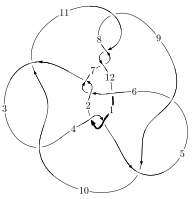
\includegraphics[width=112pt]{../../../GIT/diagram.site/Diagrams/png/1886_12a_1085.png}\\
\ \ \ A knot diagram\footnotemark}&
\allowdisplaybreaks
\textbf{Linearized knot diagam} \\
\cline{2-2}
 &
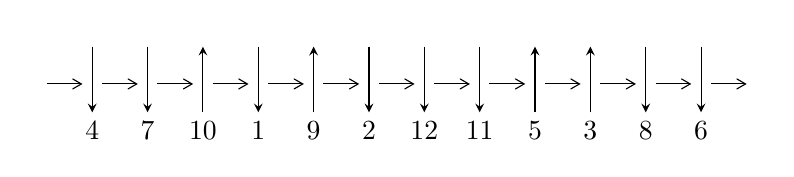
\begin{tikzpicture}[x=20pt, y=17pt]
	% nodes
	\node (C0) at (0, 0) {};
	\node (C1) at (1, 0) {};
	\node (C1U) at (1, +1) {};
	\node (C1D) at (1, -1) {4};

	\node (C2) at (2, 0) {};
	\node (C2U) at (2, +1) {};
	\node (C2D) at (2, -1) {7};

	\node (C3) at (3, 0) {};
	\node (C3U) at (3, +1) {};
	\node (C3D) at (3, -1) {10};

	\node (C4) at (4, 0) {};
	\node (C4U) at (4, +1) {};
	\node (C4D) at (4, -1) {1};

	\node (C5) at (5, 0) {};
	\node (C5U) at (5, +1) {};
	\node (C5D) at (5, -1) {9};

	\node (C6) at (6, 0) {};
	\node (C6U) at (6, +1) {};
	\node (C6D) at (6, -1) {2};

	\node (C7) at (7, 0) {};
	\node (C7U) at (7, +1) {};
	\node (C7D) at (7, -1) {12};

	\node (C8) at (8, 0) {};
	\node (C8U) at (8, +1) {};
	\node (C8D) at (8, -1) {11};

	\node (C9) at (9, 0) {};
	\node (C9U) at (9, +1) {};
	\node (C9D) at (9, -1) {5};

	\node (C10) at (10, 0) {};
	\node (C10U) at (10, +1) {};
	\node (C10D) at (10, -1) {3};

	\node (C11) at (11, 0) {};
	\node (C11U) at (11, +1) {};
	\node (C11D) at (11, -1) {8};

	\node (C12) at (12, 0) {};
	\node (C12U) at (12, +1) {};
	\node (C12D) at (12, -1) {6};
	\node (C13) at (13, 0) {};

	% arrows
	\draw[->,>={angle 60}]
	(C0) edge (C1) (C1) edge (C2) (C2) edge (C3) (C3) edge (C4) (C4) edge (C5) (C5) edge (C6) (C6) edge (C7) (C7) edge (C8) (C8) edge (C9) (C9) edge (C10) (C10) edge (C11) (C11) edge (C12) (C12) edge (C13) ;	\draw[->,>=stealth]
	(C1U) edge (C1D) (C2U) edge (C2D) (C3D) edge (C3U) (C4U) edge (C4D) (C5D) edge (C5U) (C6U) edge (C6D) (C7U) edge (C7D) (C8U) edge (C8D) (C9D) edge (C9U) (C10D) edge (C10U) (C11U) edge (C11D) (C12U) edge (C12D) ;
	\end{tikzpicture} \\
\hhline{~~} \\& 
\textbf{Solving Sequence} \\ \cline{2-2} 
 &
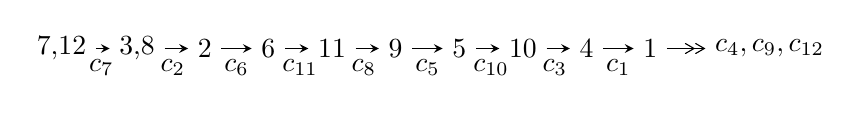
\begin{tikzpicture}[x=23pt, y=7pt]
	% node
	\node (A0) at (-1/8, 0) {7,12};
	\node (A1) at (17/16, 0) {3,8};
	\node (A2) at (17/8, 0) {2};
	\node (A3) at (25/8, 0) {6};
	\node (A4) at (33/8, 0) {11};
	\node (A5) at (41/8, 0) {9};
	\node (A6) at (49/8, 0) {5};
	\node (A7) at (57/8, 0) {10};
	\node (A8) at (65/8, 0) {4};
	\node (A9) at (73/8, 0) {1};
	\node (C1) at (1/2, -1) {$c_{7}$};
	\node (C2) at (13/8, -1) {$c_{2}$};
	\node (C3) at (21/8, -1) {$c_{6}$};
	\node (C4) at (29/8, -1) {$c_{11}$};
	\node (C5) at (37/8, -1) {$c_{8}$};
	\node (C6) at (45/8, -1) {$c_{5}$};
	\node (C7) at (53/8, -1) {$c_{10}$};
	\node (C8) at (61/8, -1) {$c_{3}$};
	\node (C9) at (69/8, -1) {$c_{1}$};
	\node (A10) at (11, 0) {$c_{4},c_{9},c_{12}$};

	% edge
	\draw[->,>=stealth]	
	(A0) edge (A1) (A1) edge (A2) (A2) edge (A3) (A3) edge (A4) (A4) edge (A5) (A5) edge (A6) (A6) edge (A7) (A7) edge (A8) (A8) edge (A9) ;
	\draw[->>,>={angle 60}]	
	(A9) edge (A10);
\end{tikzpicture} \\ 

\end{tabular} \\

\footnotetext{
The image of knot diagram is generated by the software ``\textbf{Draw programme}" developed by Andrew Bartholomew(\url{http://www.layer8.co.uk/maths/draw/index.htm\#Running-draw}), where we modified some parts for our purpose(\url{https://github.com/CATsTAILs/LinksPainter}).
}\phantom \\ \newline 
\centering \textbf{Ideals for irreducible components\footnotemark of $X_{\text{par}}$} 
 
\begin{align*}
I^u_{1}&=\langle 
-4.55506\times10^{297} u^{130}-1.07595\times10^{298} u^{129}+\cdots+3.32793\times10^{297} b+1.89111\times10^{300},\\
\phantom{I^u_{1}}&\phantom{= \langle  }3.29789\times10^{300} u^{130}+1.06460\times10^{301} u^{129}+\cdots+3.33792\times10^{300} a+2.16601\times10^{303},\\
\phantom{I^u_{1}}&\phantom{= \langle  }u^{131}+3 u^{130}+\cdots+6557 u+1003\rangle \\
I^u_{2}&=\langle 
9205 u^{37}-56551 u^{36}+\cdots+2759 b-17392,\;999 u^{37}+1035 u^{36}+\cdots+2759 a+9185,\\
\phantom{I^u_{2}}&\phantom{= \langle  }u^{38}-4 u^{37}+\cdots-8 u+1\rangle \\
\\
\end{align*}
\raggedright * 2 irreducible components of $\dim_{\mathbb{C}}=0$, with total 169 representations.\\
\footnotetext{All coefficients of polynomials are rational numbers. But the coefficients are sometimes approximated in decimal forms when there is not enough margin.}
\newpage
\renewcommand{\arraystretch}{1}
\centering \section*{I. $I^u_{1}= \langle -4.56\times10^{297} u^{130}-1.08\times10^{298} u^{129}+\cdots+3.33\times10^{297} b+1.89\times10^{300},\;3.30\times10^{300} u^{130}+1.06\times10^{301} u^{129}+\cdots+3.34\times10^{300} a+2.17\times10^{303},\;u^{131}+3 u^{130}+\cdots+6557 u+1003 \rangle$}
\flushleft \textbf{(i) Arc colorings}\\
\begin{tabular}{m{7pt} m{180pt} m{7pt} m{180pt} }
\flushright $a_{7}=$&$\begin{pmatrix}1\\0\end{pmatrix}$ \\
\flushright $a_{12}=$&$\begin{pmatrix}0\\u\end{pmatrix}$ \\
\flushright $a_{3}=$&$\begin{pmatrix}-0.988006 u^{130}-3.18941 u^{129}+\cdots-4307.93 u-648.910\\1.36873 u^{130}+3.23310 u^{129}+\cdots-2225.95 u-568.252\end{pmatrix}$ \\
\flushright $a_{8}=$&$\begin{pmatrix}1\\u^2\end{pmatrix}$ \\
\flushright $a_{2}=$&$\begin{pmatrix}0.380727 u^{130}+0.0436875 u^{129}+\cdots-6533.88 u-1217.16\\1.36873 u^{130}+3.23310 u^{129}+\cdots-2225.95 u-568.252\end{pmatrix}$ \\
\flushright $a_{6}=$&$\begin{pmatrix}0.446882 u^{130}+1.40976 u^{129}+\cdots+1941.40 u+215.692\\0.117990 u^{130}+0.692334 u^{129}+\cdots+2224.63 u+374.684\end{pmatrix}$ \\
\flushright $a_{11}=$&$\begin{pmatrix}u\\u^3+u\end{pmatrix}$ \\
\flushright $a_{9}=$&$\begin{pmatrix}u^2+1\\u^4+2 u^2\end{pmatrix}$ \\
\flushright $a_{5}=$&$\begin{pmatrix}0.593039 u^{130}+2.03783 u^{129}+\cdots+3733.75 u+516.466\\-0.0419501 u^{130}+0.305545 u^{129}+\cdots+2788.24 u+509.061\end{pmatrix}$ \\
\flushright $a_{10}=$&$\begin{pmatrix}0.452060 u^{130}+0.814581 u^{129}+\cdots+2309.50 u+589.182\\-0.102605 u^{130}+0.105061 u^{129}+\cdots+923.553 u+181.597\end{pmatrix}$ \\
\flushright $a_{4}=$&$\begin{pmatrix}-2.29003 u^{130}-5.13247 u^{129}+\cdots+6306.85 u+1492.58\\-1.98969 u^{130}-5.06913 u^{129}+\cdots+1208.27 u+424.354\end{pmatrix}$ \\
\flushright $a_{1}=$&$\begin{pmatrix}-0.365237 u^{130}-1.42252 u^{129}+\cdots-2974.24 u-244.912\\0.777842 u^{130}+1.26849 u^{129}+\cdots-5034.27 u-976.706\end{pmatrix}$\\&\end{tabular}
\flushleft \textbf{(ii) Obstruction class $= -1$}\\~\\
\flushleft \textbf{(iii) Cusp Shapes $= 0.287805 u^{130}+1.86995 u^{129}+\cdots+12047.8 u+2480.08$}\\~\\
\newpage\renewcommand{\arraystretch}{1}
\flushleft \textbf{(iv) u-Polynomials at the component}\newline \\
\begin{tabular}{m{50pt}|m{274pt}}
Crossings & \hspace{64pt}u-Polynomials at each crossing \\
\hline $$\begin{aligned}c_{1},c_{4}\end{aligned}$$&$\begin{aligned}
&u^{131}-3 u^{130}+\cdots-5 u+1
\end{aligned}$\\
\hline $$\begin{aligned}c_{2},c_{6}\end{aligned}$$&$\begin{aligned}
&u^{131}- u^{130}+\cdots+124858 u+34547
\end{aligned}$\\
\hline $$\begin{aligned}c_{3},c_{10}\end{aligned}$$&$\begin{aligned}
&u^{131}+u^{130}+\cdots-3046848 u+2207401
\end{aligned}$\\
\hline $$\begin{aligned}c_{5},c_{9}\end{aligned}$$&$\begin{aligned}
&u^{131}-3 u^{130}+\cdots-20576 u+928
\end{aligned}$\\
\hline $$\begin{aligned}c_{7},c_{8},c_{11}\end{aligned}$$&$\begin{aligned}
&u^{131}-3 u^{130}+\cdots+6557 u-1003
\end{aligned}$\\
\hline $$\begin{aligned}c_{12}\end{aligned}$$&$\begin{aligned}
&u^{131}+u^{130}+\cdots-102925 u+30725
\end{aligned}$\\
\hline
\end{tabular}\\~\\
\newpage\renewcommand{\arraystretch}{1}
\flushleft \textbf{(v) Riley Polynomials at the component}\newline \\
\begin{tabular}{m{50pt}|m{274pt}}
Crossings & \hspace{64pt}Riley Polynomials at each crossing \\
\hline $$\begin{aligned}c_{1},c_{4}\end{aligned}$$&$\begin{aligned}
&y^{131}+63 y^{130}+\cdots-95 y-1
\end{aligned}$\\
\hline $$\begin{aligned}c_{2},c_{6}\end{aligned}$$&$\begin{aligned}
&y^{131}-79 y^{130}+\cdots+24976423722 y-1193495209
\end{aligned}$\\
\hline $$\begin{aligned}c_{3},c_{10}\end{aligned}$$&$\begin{aligned}
&y^{131}+97 y^{130}+\cdots-107213854635398 y-4872619174801
\end{aligned}$\\
\hline $$\begin{aligned}c_{5},c_{9}\end{aligned}$$&$\begin{aligned}
&y^{131}+81 y^{130}+\cdots+109900800 y-861184
\end{aligned}$\\
\hline $$\begin{aligned}c_{7},c_{8},c_{11}\end{aligned}$$&$\begin{aligned}
&y^{131}+123 y^{130}+\cdots+26057591 y-1006009
\end{aligned}$\\
\hline $$\begin{aligned}c_{12}\end{aligned}$$&$\begin{aligned}
&y^{131}- y^{130}+\cdots-182071674025 y-944025625
\end{aligned}$\\
\hline
\end{tabular}\\~\\
\newpage\flushleft \textbf{(vi) Complex Volumes and Cusp Shapes}
$$\begin{array}{c|c|c}  
\text{Solutions to }I^u_{1}& \I (\text{vol} + \sqrt{-1}CS) & \text{Cusp shape}\\
 \hline 
\begin{aligned}
u &= -0.934694 + 0.329104 I \\
a &= -0.550835 - 0.743791 I \\
b &= -1.31849 + 0.55849 I\end{aligned}
 & -6.0155 + 13.7624 I & \phantom{-0.000000 } 0 \\ \hline\begin{aligned}
u &= -0.934694 - 0.329104 I \\
a &= -0.550835 + 0.743791 I \\
b &= -1.31849 - 0.55849 I\end{aligned}
 & -6.0155 - 13.7624 I & \phantom{-0.000000 } 0 \\ \hline\begin{aligned}
u &= \phantom{-}0.679855 + 0.683286 I \\
a &= -0.462761 - 0.629021 I \\
b &= \phantom{-}1.131680 - 0.277058 I\end{aligned}
 & -1.55411 + 2.60636 I & \phantom{-0.000000 } 0 \\ \hline\begin{aligned}
u &= \phantom{-}0.679855 - 0.683286 I \\
a &= -0.462761 + 0.629021 I \\
b &= \phantom{-}1.131680 + 0.277058 I\end{aligned}
 & -1.55411 - 2.60636 I & \phantom{-0.000000 } 0 \\ \hline\begin{aligned}
u &= -1.007500 + 0.249395 I \\
a &= \phantom{-}0.528639 + 0.553378 I \\
b &= \phantom{-}1.197060 - 0.485687 I\end{aligned}
 & -8.29895 + 6.75694 I & \phantom{-0.000000 } 0 \\ \hline\begin{aligned}
u &= -1.007500 - 0.249395 I \\
a &= \phantom{-}0.528639 - 0.553378 I \\
b &= \phantom{-}1.197060 + 0.485687 I\end{aligned}
 & -8.29895 - 6.75694 I & \phantom{-0.000000 } 0 \\ \hline\begin{aligned}
u &= -0.609549 + 0.880930 I \\
a &= \phantom{-}1.033680 + 0.650673 I \\
b &= \phantom{-}0.538625 - 0.320977 I\end{aligned}
 & -3.78924 + 2.21930 I & \phantom{-0.000000 } 0 \\ \hline\begin{aligned}
u &= -0.609549 - 0.880930 I \\
a &= \phantom{-}1.033680 - 0.650673 I \\
b &= \phantom{-}0.538625 + 0.320977 I\end{aligned}
 & -3.78924 - 2.21930 I & \phantom{-0.000000 } 0 \\ \hline\begin{aligned}
u &= \phantom{-}0.818465 + 0.409101 I \\
a &= -0.333227 + 0.716166 I \\
b &= -1.258220 - 0.258704 I\end{aligned}
 & -4.60969 - 2.75132 I & \phantom{-0.000000 } 0 \\ \hline\begin{aligned}
u &= \phantom{-}0.818465 - 0.409101 I \\
a &= -0.333227 - 0.716166 I \\
b &= -1.258220 + 0.258704 I\end{aligned}
 & -4.60969 + 2.75132 I & \phantom{-0.000000 } 0\\
 \hline 
 \end{array}$$\newpage$$\begin{array}{c|c|c}  
\text{Solutions to }I^u_{1}& \I (\text{vol} + \sqrt{-1}CS) & \text{Cusp shape}\\
 \hline 
\begin{aligned}
u &= \phantom{-}0.769460 + 0.454615 I \\
a &= -0.430525 + 0.833443 I \\
b &= -1.278700 - 0.122735 I\end{aligned}
 & -4.55934 - 2.49188 I & \phantom{-0.000000 } 0 \\ \hline\begin{aligned}
u &= \phantom{-}0.769460 - 0.454615 I \\
a &= -0.430525 - 0.833443 I \\
b &= -1.278700 + 0.122735 I\end{aligned}
 & -4.55934 + 2.49188 I & \phantom{-0.000000 } 0 \\ \hline\begin{aligned}
u &= \phantom{-}0.688328 + 0.873746 I \\
a &= -0.592425 + 0.433927 I \\
b &= -0.861384 + 0.124540 I\end{aligned}
 & -3.06768 - 2.44235 I & \phantom{-0.000000 } 0 \\ \hline\begin{aligned}
u &= \phantom{-}0.688328 - 0.873746 I \\
a &= -0.592425 - 0.433927 I \\
b &= -0.861384 - 0.124540 I\end{aligned}
 & -3.06768 + 2.44235 I & \phantom{-0.000000 } 0 \\ \hline\begin{aligned}
u &= \phantom{-}0.789233 + 0.386969 I \\
a &= \phantom{-}0.349506 - 0.813447 I \\
b &= \phantom{-}1.297670 + 0.546358 I\end{aligned}
 & -2.45784 - 7.50441 I & \phantom{-0.000000 } 0 \\ \hline\begin{aligned}
u &= \phantom{-}0.789233 - 0.386969 I \\
a &= \phantom{-}0.349506 + 0.813447 I \\
b &= \phantom{-}1.297670 - 0.546358 I\end{aligned}
 & -2.45784 + 7.50441 I & \phantom{-0.000000 } 0 \\ \hline\begin{aligned}
u &= -0.035834 + 1.125340 I \\
a &= -0.86865 - 2.41662 I \\
b &= \phantom{-}0.666170 + 0.860764 I\end{aligned}
 & -0.31847 - 5.32965 I & \phantom{-0.000000 } 0 \\ \hline\begin{aligned}
u &= -0.035834 - 1.125340 I \\
a &= -0.86865 + 2.41662 I \\
b &= \phantom{-}0.666170 - 0.860764 I\end{aligned}
 & -0.31847 + 5.32965 I & \phantom{-0.000000 } 0 \\ \hline\begin{aligned}
u &= -0.031587 + 1.145130 I \\
a &= \phantom{-}0.35907 + 2.14111 I \\
b &= -0.848661 - 0.423254 I\end{aligned}
 & -3.53022 + 0.23230 I & \phantom{-0.000000 } 0 \\ \hline\begin{aligned}
u &= -0.031587 - 1.145130 I \\
a &= \phantom{-}0.35907 - 2.14111 I \\
b &= -0.848661 + 0.423254 I\end{aligned}
 & -3.53022 - 0.23230 I & \phantom{-0.000000 } 0\\
 \hline 
 \end{array}$$\newpage$$\begin{array}{c|c|c}  
\text{Solutions to }I^u_{1}& \I (\text{vol} + \sqrt{-1}CS) & \text{Cusp shape}\\
 \hline 
\begin{aligned}
u &= \phantom{-}0.752508 + 0.352699 I \\
a &= -0.984423 + 0.573636 I \\
b &= -1.134740 - 0.157369 I\end{aligned}
 & -4.22971 - 2.52046 I & \phantom{-0.000000 } 0 \\ \hline\begin{aligned}
u &= \phantom{-}0.752508 - 0.352699 I \\
a &= -0.984423 - 0.573636 I \\
b &= -1.134740 + 0.157369 I\end{aligned}
 & -4.22971 + 2.52046 I & \phantom{-0.000000 } 0 \\ \hline\begin{aligned}
u &= \phantom{-}0.025206 + 1.187290 I \\
a &= \phantom{-}0.34341 - 2.21812 I \\
b &= \phantom{-}0.742032 + 0.026090 I\end{aligned}
 & \phantom{-}0.21152 + 5.29954 I & \phantom{-0.000000 } 0 \\ \hline\begin{aligned}
u &= \phantom{-}0.025206 - 1.187290 I \\
a &= \phantom{-}0.34341 + 2.21812 I \\
b &= \phantom{-}0.742032 - 0.026090 I\end{aligned}
 & \phantom{-}0.21152 - 5.29954 I & \phantom{-0.000000 } 0 \\ \hline\begin{aligned}
u &= -0.131118 + 1.184340 I \\
a &= \phantom{-}0.907058 + 0.602299 I \\
b &= -1.55156 - 0.34705 I\end{aligned}
 & -5.46941 + 0.66431 I & \phantom{-0.000000 } 0 \\ \hline\begin{aligned}
u &= -0.131118 - 1.184340 I \\
a &= \phantom{-}0.907058 - 0.602299 I \\
b &= -1.55156 + 0.34705 I\end{aligned}
 & -5.46941 - 0.66431 I & \phantom{-0.000000 } 0 \\ \hline\begin{aligned}
u &= -0.717221 + 0.957662 I \\
a &= \phantom{-}0.401088 - 0.263128 I \\
b &= -1.194890 - 0.413863 I\end{aligned}
 & -4.17251 - 8.11451 I & \phantom{-0.000000 } 0 \\ \hline\begin{aligned}
u &= -0.717221 - 0.957662 I \\
a &= \phantom{-}0.401088 + 0.263128 I \\
b &= -1.194890 + 0.413863 I\end{aligned}
 & -4.17251 + 8.11451 I & \phantom{-0.000000 } 0 \\ \hline\begin{aligned}
u &= -0.798624 + 0.068130 I \\
a &= -0.707332 + 0.137978 I \\
b &= -0.811384 - 0.753650 I\end{aligned}
 & \phantom{-}0.96424 - 2.83403 I & \phantom{-0.000000 } 0 \\ \hline\begin{aligned}
u &= -0.798624 - 0.068130 I \\
a &= -0.707332 - 0.137978 I \\
b &= -0.811384 + 0.753650 I\end{aligned}
 & \phantom{-}0.96424 + 2.83403 I & \phantom{-0.000000 } 0\\
 \hline 
 \end{array}$$\newpage$$\begin{array}{c|c|c}  
\text{Solutions to }I^u_{1}& \I (\text{vol} + \sqrt{-1}CS) & \text{Cusp shape}\\
 \hline 
\begin{aligned}
u &= \phantom{-}0.841415 + 0.864267 I \\
a &= \phantom{-}0.123708 + 0.437579 I \\
b &= -1.046930 + 0.038601 I\end{aligned}
 & -3.66191 - 2.86764 I & \phantom{-0.000000 } 0 \\ \hline\begin{aligned}
u &= \phantom{-}0.841415 - 0.864267 I \\
a &= \phantom{-}0.123708 - 0.437579 I \\
b &= -1.046930 - 0.038601 I\end{aligned}
 & -3.66191 + 2.86764 I & \phantom{-0.000000 } 0 \\ \hline\begin{aligned}
u &= -0.170127 + 1.208950 I \\
a &= -1.147570 + 0.063788 I \\
b &= \phantom{-}1.73263 + 0.21832 I\end{aligned}
 & -3.89869 + 4.95633 I & \phantom{-0.000000 } 0 \\ \hline\begin{aligned}
u &= -0.170127 - 1.208950 I \\
a &= -1.147570 - 0.063788 I \\
b &= \phantom{-}1.73263 - 0.21832 I\end{aligned}
 & -3.89869 - 4.95633 I & \phantom{-0.000000 } 0 \\ \hline\begin{aligned}
u &= \phantom{-}0.552137 + 0.539168 I \\
a &= -0.601591 + 0.174461 I \\
b &= \phantom{-}0.307493 - 0.623301 I\end{aligned}
 & \phantom{-}0.68998 - 3.26031 I & \phantom{-0.000000 } 0 \\ \hline\begin{aligned}
u &= \phantom{-}0.552137 - 0.539168 I \\
a &= -0.601591 - 0.174461 I \\
b &= \phantom{-}0.307493 + 0.623301 I\end{aligned}
 & \phantom{-}0.68998 + 3.26031 I & \phantom{-0.000000 } 0 \\ \hline\begin{aligned}
u &= -0.084779 + 1.233320 I \\
a &= -0.277224 + 0.582683 I \\
b &= -1.388380 - 0.064832 I\end{aligned}
 & -4.78082 + 1.55259 I & \phantom{-0.000000 } 0 \\ \hline\begin{aligned}
u &= -0.084779 - 1.233320 I \\
a &= -0.277224 - 0.582683 I \\
b &= -1.388380 + 0.064832 I\end{aligned}
 & -4.78082 - 1.55259 I & \phantom{-0.000000 } 0 \\ \hline\begin{aligned}
u &= -0.697567 + 0.288833 I \\
a &= \phantom{-}0.509289 - 0.451238 I \\
b &= \phantom{-}0.092417 + 0.707095 I\end{aligned}
 & -5.12293 + 2.23297 I & \phantom{-0.000000 } 0 \\ \hline\begin{aligned}
u &= -0.697567 - 0.288833 I \\
a &= \phantom{-}0.509289 + 0.451238 I \\
b &= \phantom{-}0.092417 - 0.707095 I\end{aligned}
 & -5.12293 - 2.23297 I & \phantom{-0.000000 } 0\\
 \hline 
 \end{array}$$\newpage$$\begin{array}{c|c|c}  
\text{Solutions to }I^u_{1}& \I (\text{vol} + \sqrt{-1}CS) & \text{Cusp shape}\\
 \hline 
\begin{aligned}
u &= -0.119894 + 1.260100 I \\
a &= \phantom{-}0.090350 + 0.352826 I \\
b &= \phantom{-}1.56261 + 0.03072 I\end{aligned}
 & -3.04352 - 1.72138 I & \phantom{-0.000000 } 0 \\ \hline\begin{aligned}
u &= -0.119894 - 1.260100 I \\
a &= \phantom{-}0.090350 - 0.352826 I \\
b &= \phantom{-}1.56261 - 0.03072 I\end{aligned}
 & -3.04352 + 1.72138 I & \phantom{-0.000000 } 0 \\ \hline\begin{aligned}
u &= -0.667494 + 0.272419 I \\
a &= -0.174243 + 0.449009 I \\
b &= -0.053870 - 1.094810 I\end{aligned}
 & -2.09095 + 7.97659 I & \phantom{-0.000000 } 0 \\ \hline\begin{aligned}
u &= -0.667494 - 0.272419 I \\
a &= -0.174243 - 0.449009 I \\
b &= -0.053870 + 1.094810 I\end{aligned}
 & -2.09095 - 7.97659 I & \phantom{-0.000000 } 0 \\ \hline\begin{aligned}
u &= \phantom{-}0.545298 + 0.467803 I \\
a &= \phantom{-}0.571463 + 0.100897 I \\
b &= \phantom{-}0.938446 - 0.555977 I\end{aligned}
 & -1.20051 + 3.65561 I & \phantom{-0.000000 } 0 \\ \hline\begin{aligned}
u &= \phantom{-}0.545298 - 0.467803 I \\
a &= \phantom{-}0.571463 - 0.100897 I \\
b &= \phantom{-}0.938446 + 0.555977 I\end{aligned}
 & -1.20051 - 3.65561 I & \phantom{-0.000000 } 0 \\ \hline\begin{aligned}
u &= -0.458111 + 0.528404 I \\
a &= -1.86536 - 0.22014 I \\
b &= -0.200295 + 0.463592 I\end{aligned}
 & -1.05071 - 4.43531 I & \phantom{-0.000000 } 0 \\ \hline\begin{aligned}
u &= -0.458111 - 0.528404 I \\
a &= -1.86536 + 0.22014 I \\
b &= -0.200295 - 0.463592 I\end{aligned}
 & -1.05071 + 4.43531 I & \phantom{-0.000000 } 0 \\ \hline\begin{aligned}
u &= \phantom{-}0.615847 + 0.313571 I \\
a &= \phantom{-}1.88745 - 0.94174 I \\
b &= \phantom{-}1.102450 + 0.400010 I\end{aligned}
 & -1.65081 - 7.22240 I & -7.00170 + 8.40269 I \\ \hline\begin{aligned}
u &= \phantom{-}0.615847 - 0.313571 I \\
a &= \phantom{-}1.88745 + 0.94174 I \\
b &= \phantom{-}1.102450 - 0.400010 I\end{aligned}
 & -1.65081 + 7.22240 I & -7.00170 - 8.40269 I\\
 \hline 
 \end{array}$$\newpage$$\begin{array}{c|c|c}  
\text{Solutions to }I^u_{1}& \I (\text{vol} + \sqrt{-1}CS) & \text{Cusp shape}\\
 \hline 
\begin{aligned}
u &= \phantom{-}0.595933 + 0.324234 I \\
a &= \phantom{-}0.461656 - 0.734192 I \\
b &= \phantom{-}0.389923 + 0.502982 I\end{aligned}
 & \phantom{-}0.111356 - 0.603783 I & -4.00000 + 2.81913 I \\ \hline\begin{aligned}
u &= \phantom{-}0.595933 - 0.324234 I \\
a &= \phantom{-}0.461656 + 0.734192 I \\
b &= \phantom{-}0.389923 - 0.502982 I\end{aligned}
 & \phantom{-}0.111356 + 0.603783 I & -4.00000 - 2.81913 I \\ \hline\begin{aligned}
u &= \phantom{-}0.135341 + 1.316130 I \\
a &= \phantom{-}0.35019 - 2.02274 I \\
b &= -0.26473 + 1.40134 I\end{aligned}
 & \phantom{-}5.28796 - 0.51685 I & \phantom{-0.000000 } 0 \\ \hline\begin{aligned}
u &= \phantom{-}0.135341 - 1.316130 I \\
a &= \phantom{-}0.35019 + 2.02274 I \\
b &= -0.26473 - 1.40134 I\end{aligned}
 & \phantom{-}5.28796 + 0.51685 I & \phantom{-0.000000 } 0 \\ \hline\begin{aligned}
u &= -0.684844 + 1.155350 I \\
a &= -0.353479 + 0.149555 I \\
b &= \phantom{-}1.072870 + 0.356066 I\end{aligned}
 & -5.62717 - 0.84114 I & \phantom{-0.000000 } 0 \\ \hline\begin{aligned}
u &= -0.684844 - 1.155350 I \\
a &= -0.353479 - 0.149555 I \\
b &= \phantom{-}1.072870 - 0.356066 I\end{aligned}
 & -5.62717 + 0.84114 I & \phantom{-0.000000 } 0 \\ \hline\begin{aligned}
u &= -0.140360 + 1.349520 I \\
a &= -0.201290 + 1.328550 I \\
b &= \phantom{-}1.116370 - 0.449257 I\end{aligned}
 & \phantom{-}2.62547 + 1.91932 I & \phantom{-0.000000 } 0 \\ \hline\begin{aligned}
u &= -0.140360 - 1.349520 I \\
a &= -0.201290 - 1.328550 I \\
b &= \phantom{-}1.116370 + 0.449257 I\end{aligned}
 & \phantom{-}2.62547 - 1.91932 I & \phantom{-0.000000 } 0 \\ \hline\begin{aligned}
u &= \phantom{-}0.179299 + 1.349430 I \\
a &= -0.80224 + 1.81570 I \\
b &= \phantom{-}0.64697 - 1.39086 I\end{aligned}
 & \phantom{-}5.93037 - 3.80995 I & \phantom{-0.000000 } 0 \\ \hline\begin{aligned}
u &= \phantom{-}0.179299 - 1.349430 I \\
a &= -0.80224 - 1.81570 I \\
b &= \phantom{-}0.64697 + 1.39086 I\end{aligned}
 & \phantom{-}5.93037 + 3.80995 I & \phantom{-0.000000 } 0\\
 \hline 
 \end{array}$$\newpage$$\begin{array}{c|c|c}  
\text{Solutions to }I^u_{1}& \I (\text{vol} + \sqrt{-1}CS) & \text{Cusp shape}\\
 \hline 
\begin{aligned}
u &= \phantom{-}0.276716 + 1.333720 I \\
a &= \phantom{-}0.318553 - 0.745790 I \\
b &= \phantom{-}1.064700 + 0.376173 I\end{aligned}
 & \phantom{-}4.72117 - 2.74730 I & \phantom{-0.000000 } 0 \\ \hline\begin{aligned}
u &= \phantom{-}0.276716 - 1.333720 I \\
a &= \phantom{-}0.318553 + 0.745790 I \\
b &= \phantom{-}1.064700 - 0.376173 I\end{aligned}
 & \phantom{-}4.72117 + 2.74730 I & \phantom{-0.000000 } 0 \\ \hline\begin{aligned}
u &= -0.395334 + 1.305160 I \\
a &= -0.36074 - 1.63019 I \\
b &= -0.960863 + 0.772999 I\end{aligned}
 & \phantom{-}4.85292 + 7.20961 I & \phantom{-0.000000 } 0 \\ \hline\begin{aligned}
u &= -0.395334 - 1.305160 I \\
a &= -0.36074 + 1.63019 I \\
b &= -0.960863 - 0.772999 I\end{aligned}
 & \phantom{-}4.85292 - 7.20961 I & \phantom{-0.000000 } 0 \\ \hline\begin{aligned}
u &= \phantom{-}0.635440 + 0.006329 I \\
a &= \phantom{-}1.09310 - 1.01779 I \\
b &= \phantom{-}0.590265 - 0.091851 I\end{aligned}
 & \phantom{-}0.443485 - 0.658778 I & -6.88794 - 0.16623 I \\ \hline\begin{aligned}
u &= \phantom{-}0.635440 - 0.006329 I \\
a &= \phantom{-}1.09310 + 1.01779 I \\
b &= \phantom{-}0.590265 + 0.091851 I\end{aligned}
 & \phantom{-}0.443485 + 0.658778 I & -6.88794 + 0.16623 I \\ \hline\begin{aligned}
u &= -0.602014 + 0.190107 I \\
a &= -0.117972 - 1.364090 I \\
b &= -1.189610 + 0.529459 I\end{aligned}
 & -8.28202 + 1.92303 I & -12.09420 - 6.84885 I \\ \hline\begin{aligned}
u &= -0.602014 - 0.190107 I \\
a &= -0.117972 + 1.364090 I \\
b &= -1.189610 - 0.529459 I\end{aligned}
 & -8.28202 - 1.92303 I & -12.09420 + 6.84885 I \\ \hline\begin{aligned}
u &= -0.236766 + 1.349600 I \\
a &= -0.95781 + 1.84822 I \\
b &= \phantom{-}1.27816 - 0.66979 I\end{aligned}
 & -2.40209 + 0.83917 I & \phantom{-0.000000 } 0 \\ \hline\begin{aligned}
u &= -0.236766 - 1.349600 I \\
a &= -0.95781 - 1.84822 I \\
b &= \phantom{-}1.27816 + 0.66979 I\end{aligned}
 & -2.40209 - 0.83917 I & \phantom{-0.000000 } 0\\
 \hline 
 \end{array}$$\newpage$$\begin{array}{c|c|c}  
\text{Solutions to }I^u_{1}& \I (\text{vol} + \sqrt{-1}CS) & \text{Cusp shape}\\
 \hline 
\begin{aligned}
u &= \phantom{-}0.097821 + 1.371550 I \\
a &= \phantom{-}0.081815 - 1.219470 I \\
b &= -0.347833 + 0.449614 I\end{aligned}
 & \phantom{-}4.86122 - 2.83742 I & \phantom{-0.000000 } 0 \\ \hline\begin{aligned}
u &= \phantom{-}0.097821 - 1.371550 I \\
a &= \phantom{-}0.081815 + 1.219470 I \\
b &= -0.347833 - 0.449614 I\end{aligned}
 & \phantom{-}4.86122 + 2.83742 I & \phantom{-0.000000 } 0 \\ \hline\begin{aligned}
u &= -0.182001 + 1.368620 I \\
a &= \phantom{-}0.10079 - 1.69592 I \\
b &= -1.214110 + 0.687059 I\end{aligned}
 & \phantom{-}6.96416 + 5.92527 I & \phantom{-0.000000 } 0 \\ \hline\begin{aligned}
u &= -0.182001 - 1.368620 I \\
a &= \phantom{-}0.10079 + 1.69592 I \\
b &= -1.214110 - 0.687059 I\end{aligned}
 & \phantom{-}6.96416 - 5.92527 I & \phantom{-0.000000 } 0 \\ \hline\begin{aligned}
u &= -0.598169 + 0.129833 I \\
a &= \phantom{-}0.550974 + 1.159430 I \\
b &= \phantom{-}1.48357 - 0.42359 I\end{aligned}
 & -7.10762 - 2.21508 I & -10.60536 + 2.23170 I \\ \hline\begin{aligned}
u &= -0.598169 - 0.129833 I \\
a &= \phantom{-}0.550974 - 1.159430 I \\
b &= \phantom{-}1.48357 + 0.42359 I\end{aligned}
 & -7.10762 + 2.21508 I & -10.60536 - 2.23170 I \\ \hline\begin{aligned}
u &= -0.190570 + 1.375840 I \\
a &= -1.07455 + 1.87376 I \\
b &= \phantom{-}1.152520 - 0.159315 I\end{aligned}
 & -1.53807 + 6.24014 I & \phantom{-0.000000 } 0 \\ \hline\begin{aligned}
u &= -0.190570 - 1.375840 I \\
a &= -1.07455 - 1.87376 I \\
b &= \phantom{-}1.152520 + 0.159315 I\end{aligned}
 & -1.53807 - 6.24014 I & \phantom{-0.000000 } 0 \\ \hline\begin{aligned}
u &= -0.294482 + 1.363240 I \\
a &= \phantom{-}0.756292 + 0.710811 I \\
b &= -0.727685 - 0.916619 I\end{aligned}
 & \phantom{-}5.57411 + 1.03954 I & \phantom{-0.000000 } 0 \\ \hline\begin{aligned}
u &= -0.294482 - 1.363240 I \\
a &= \phantom{-}0.756292 - 0.710811 I \\
b &= -0.727685 + 0.916619 I\end{aligned}
 & \phantom{-}5.57411 - 1.03954 I & \phantom{-0.000000 } 0\\
 \hline 
 \end{array}$$\newpage$$\begin{array}{c|c|c}  
\text{Solutions to }I^u_{1}& \I (\text{vol} + \sqrt{-1}CS) & \text{Cusp shape}\\
 \hline 
\begin{aligned}
u &= -0.245737 + 1.376050 I \\
a &= \phantom{-}0.76197 - 1.82749 I \\
b &= -0.944287 + 0.769941 I\end{aligned}
 & -3.28024 + 5.04757 I & \phantom{-0.000000 } 0 \\ \hline\begin{aligned}
u &= -0.245737 - 1.376050 I \\
a &= \phantom{-}0.76197 + 1.82749 I \\
b &= -0.944287 - 0.769941 I\end{aligned}
 & -3.28024 - 5.04757 I & \phantom{-0.000000 } 0 \\ \hline\begin{aligned}
u &= -0.20359 + 1.40017 I \\
a &= \phantom{-}1.14728 - 1.56629 I \\
b &= -0.840553 + 0.145478 I\end{aligned}
 & -2.49420 + 2.92894 I & \phantom{-0.000000 } 0 \\ \hline\begin{aligned}
u &= -0.20359 - 1.40017 I \\
a &= \phantom{-}1.14728 + 1.56629 I \\
b &= -0.840553 - 0.145478 I\end{aligned}
 & -2.49420 - 2.92894 I & \phantom{-0.000000 } 0 \\ \hline\begin{aligned}
u &= -0.09468 + 1.41900 I \\
a &= -0.136059 - 1.064040 I \\
b &= -0.818408 + 0.488902 I\end{aligned}
 & \phantom{-}5.40126 - 2.73374 I & \phantom{-0.000000 } 0 \\ \hline\begin{aligned}
u &= -0.09468 - 1.41900 I \\
a &= -0.136059 + 1.064040 I \\
b &= -0.818408 - 0.488902 I\end{aligned}
 & \phantom{-}5.40126 + 2.73374 I & \phantom{-0.000000 } 0 \\ \hline\begin{aligned}
u &= -0.27503 + 1.40354 I \\
a &= -0.390920 - 1.279640 I \\
b &= \phantom{-}0.249244 + 1.055930 I\end{aligned}
 & \phantom{-}0.23806 + 5.77413 I & \phantom{-0.000000 } 0 \\ \hline\begin{aligned}
u &= -0.27503 - 1.40354 I \\
a &= -0.390920 + 1.279640 I \\
b &= \phantom{-}0.249244 - 1.055930 I\end{aligned}
 & \phantom{-}0.23806 - 5.77413 I & \phantom{-0.000000 } 0 \\ \hline\begin{aligned}
u &= -0.26689 + 1.40609 I \\
a &= \phantom{-}0.61770 + 1.56594 I \\
b &= -0.263332 - 1.335610 I\end{aligned}
 & \phantom{-}3.26018 + 11.39960 I & \phantom{-0.000000 } 0 \\ \hline\begin{aligned}
u &= -0.26689 - 1.40609 I \\
a &= \phantom{-}0.61770 - 1.56594 I \\
b &= -0.263332 + 1.335610 I\end{aligned}
 & \phantom{-}3.26018 - 11.39960 I & \phantom{-0.000000 } 0\\
 \hline 
 \end{array}$$\newpage$$\begin{array}{c|c|c}  
\text{Solutions to }I^u_{1}& \I (\text{vol} + \sqrt{-1}CS) & \text{Cusp shape}\\
 \hline 
\begin{aligned}
u &= \phantom{-}0.24673 + 1.41926 I \\
a &= \phantom{-}0.15074 - 1.55465 I \\
b &= \phantom{-}1.283560 + 0.468672 I\end{aligned}
 & \phantom{-}3.88495 - 10.41490 I & \phantom{-0.000000 } 0 \\ \hline\begin{aligned}
u &= \phantom{-}0.24673 - 1.41926 I \\
a &= \phantom{-}0.15074 + 1.55465 I \\
b &= \phantom{-}1.283560 - 0.468672 I\end{aligned}
 & \phantom{-}3.88495 + 10.41490 I & \phantom{-0.000000 } 0 \\ \hline\begin{aligned}
u &= \phantom{-}0.29309 + 1.41111 I \\
a &= -0.00538 - 1.49492 I \\
b &= \phantom{-}0.763063 + 0.589715 I\end{aligned}
 & \phantom{-}5.39679 - 4.00449 I & \phantom{-0.000000 } 0 \\ \hline\begin{aligned}
u &= \phantom{-}0.29309 - 1.41111 I \\
a &= -0.00538 + 1.49492 I \\
b &= \phantom{-}0.763063 - 0.589715 I\end{aligned}
 & \phantom{-}5.39679 + 4.00449 I & \phantom{-0.000000 } 0 \\ \hline\begin{aligned}
u &= \phantom{-}0.09209 + 1.44027 I \\
a &= -0.009980 - 1.173310 I \\
b &= \phantom{-}0.077908 + 0.755724 I\end{aligned}
 & \phantom{-}5.60105 - 2.33906 I & \phantom{-0.000000 } 0 \\ \hline\begin{aligned}
u &= \phantom{-}0.09209 - 1.44027 I \\
a &= -0.009980 + 1.173310 I \\
b &= \phantom{-}0.077908 - 0.755724 I\end{aligned}
 & \phantom{-}5.60105 + 2.33906 I & \phantom{-0.000000 } 0 \\ \hline\begin{aligned}
u &= -0.05220 + 1.44278 I \\
a &= \phantom{-}0.76947 + 1.22543 I \\
b &= -0.481725 - 1.001430 I\end{aligned}
 & \phantom{-}9.36512 - 0.24380 I & \phantom{-0.000000 } 0 \\ \hline\begin{aligned}
u &= -0.05220 - 1.44278 I \\
a &= \phantom{-}0.76947 - 1.22543 I \\
b &= -0.481725 + 1.001430 I\end{aligned}
 & \phantom{-}9.36512 + 0.24380 I & \phantom{-0.000000 } 0 \\ \hline\begin{aligned}
u &= \phantom{-}0.15627 + 1.44707 I \\
a &= -0.665878 + 0.986739 I \\
b &= \phantom{-}0.885210 - 0.764178 I\end{aligned}
 & \phantom{-}5.06496 + 1.24276 I & \phantom{-0.000000 } 0 \\ \hline\begin{aligned}
u &= \phantom{-}0.15627 - 1.44707 I \\
a &= -0.665878 - 0.986739 I \\
b &= \phantom{-}0.885210 + 0.764178 I\end{aligned}
 & \phantom{-}5.06496 - 1.24276 I & \phantom{-0.000000 } 0\\
 \hline 
 \end{array}$$\newpage$$\begin{array}{c|c|c}  
\text{Solutions to }I^u_{1}& \I (\text{vol} + \sqrt{-1}CS) & \text{Cusp shape}\\
 \hline 
\begin{aligned}
u &= -0.493511 + 0.222405 I \\
a &= \phantom{-}0.27867 - 2.67640 I \\
b &= -1.098540 + 0.009317 I\end{aligned}
 & -7.73990 + 0.30324 I & -10.22397 + 1.81420 I \\ \hline\begin{aligned}
u &= -0.493511 - 0.222405 I \\
a &= \phantom{-}0.27867 + 2.67640 I \\
b &= -1.098540 - 0.009317 I\end{aligned}
 & -7.73990 - 0.30324 I & -10.22397 - 1.81420 I \\ \hline\begin{aligned}
u &= \phantom{-}0.30264 + 1.43258 I \\
a &= \phantom{-}0.261994 + 1.189960 I \\
b &= -1.271090 - 0.348276 I\end{aligned}
 & \phantom{-}1.44040 - 6.34992 I & \phantom{-0.000000 } 0 \\ \hline\begin{aligned}
u &= \phantom{-}0.30264 - 1.43258 I \\
a &= \phantom{-}0.261994 - 1.189960 I \\
b &= -1.271090 + 0.348276 I\end{aligned}
 & \phantom{-}1.44040 + 6.34992 I & \phantom{-0.000000 } 0 \\ \hline\begin{aligned}
u &= -0.487402 + 0.179252 I \\
a &= -1.76300 - 0.40363 I \\
b &= -0.955363 + 0.526859 I\end{aligned}
 & \phantom{-}2.04111 + 3.47849 I & \phantom{-}0.98681 - 5.99163 I \\ \hline\begin{aligned}
u &= -0.487402 - 0.179252 I \\
a &= -1.76300 + 0.40363 I \\
b &= -0.955363 - 0.526859 I\end{aligned}
 & \phantom{-}2.04111 - 3.47849 I & \phantom{-}0.98681 + 5.99163 I \\ \hline\begin{aligned}
u &= \phantom{-}0.29366 + 1.45267 I \\
a &= \phantom{-}0.345081 + 1.327240 I \\
b &= -1.280140 - 0.348591 I\end{aligned}
 & \phantom{-}1.46725 - 6.38484 I & \phantom{-0.000000 } 0 \\ \hline\begin{aligned}
u &= \phantom{-}0.29366 - 1.45267 I \\
a &= \phantom{-}0.345081 - 1.327240 I \\
b &= -1.280140 + 0.348591 I\end{aligned}
 & \phantom{-}1.46725 + 6.38484 I & \phantom{-0.000000 } 0 \\ \hline\begin{aligned}
u &= -0.235458 + 0.457864 I \\
a &= \phantom{-}0.621199 - 0.179878 I \\
b &= -0.554225 - 0.747913 I\end{aligned}
 & \phantom{-}3.24807 - 1.24361 I & \phantom{-}3.59115 + 1.44966 I \\ \hline\begin{aligned}
u &= -0.235458 - 0.457864 I \\
a &= \phantom{-}0.621199 + 0.179878 I \\
b &= -0.554225 + 0.747913 I\end{aligned}
 & \phantom{-}3.24807 + 1.24361 I & \phantom{-}3.59115 - 1.44966 I\\
 \hline 
 \end{array}$$\newpage$$\begin{array}{c|c|c}  
\text{Solutions to }I^u_{1}& \I (\text{vol} + \sqrt{-1}CS) & \text{Cusp shape}\\
 \hline 
\begin{aligned}
u &= \phantom{-}0.31495 + 1.45741 I \\
a &= \phantom{-}0.50195 + 1.43358 I \\
b &= -1.278780 - 0.542741 I\end{aligned}
 & \phantom{-}1.31586 - 6.84522 I & \phantom{-0.000000 } 0 \\ \hline\begin{aligned}
u &= \phantom{-}0.31495 - 1.45741 I \\
a &= \phantom{-}0.50195 - 1.43358 I \\
b &= -1.278780 + 0.542741 I\end{aligned}
 & \phantom{-}1.31586 + 6.84522 I & \phantom{-0.000000 } 0 \\ \hline\begin{aligned}
u &= \phantom{-}0.30653 + 1.46274 I \\
a &= -0.52357 - 1.71904 I \\
b &= \phantom{-}1.30238 + 0.79237 I\end{aligned}
 & \phantom{-}3.46299 - 11.48740 I & \phantom{-0.000000 } 0 \\ \hline\begin{aligned}
u &= \phantom{-}0.30653 - 1.46274 I \\
a &= -0.52357 + 1.71904 I \\
b &= \phantom{-}1.30238 - 0.79237 I\end{aligned}
 & \phantom{-}3.46299 + 11.48740 I & \phantom{-0.000000 } 0 \\ \hline\begin{aligned}
u &= -0.479468 + 0.147171 I \\
a &= \phantom{-}1.22541 + 2.78516 I \\
b &= \phantom{-}1.363860 - 0.031652 I\end{aligned}
 & -6.46178 + 3.74739 I & -12.72826 - 5.14170 I \\ \hline\begin{aligned}
u &= -0.479468 - 0.147171 I \\
a &= \phantom{-}1.22541 - 2.78516 I \\
b &= \phantom{-}1.363860 + 0.031652 I\end{aligned}
 & -6.46178 - 3.74739 I & -12.72826 + 5.14170 I \\ \hline\begin{aligned}
u &= -0.41159 + 1.44962 I \\
a &= -0.18195 + 1.55187 I \\
b &= \phantom{-}1.263230 - 0.632475 I\end{aligned}
 & -2.88992 + 11.81910 I & \phantom{-0.000000 } 0 \\ \hline\begin{aligned}
u &= -0.41159 - 1.44962 I \\
a &= -0.18195 - 1.55187 I \\
b &= \phantom{-}1.263230 + 0.632475 I\end{aligned}
 & -2.88992 - 11.81910 I & \phantom{-0.000000 } 0 \\ \hline\begin{aligned}
u &= -0.37251 + 1.46706 I \\
a &= \phantom{-}0.30220 - 1.72005 I \\
b &= -1.36377 + 0.69905 I\end{aligned}
 & -0.2841 + 18.4649 I & \phantom{-0.000000 } 0 \\ \hline\begin{aligned}
u &= -0.37251 - 1.46706 I \\
a &= \phantom{-}0.30220 + 1.72005 I \\
b &= -1.36377 - 0.69905 I\end{aligned}
 & -0.2841 - 18.4649 I & \phantom{-0.000000 } 0\\
 \hline 
 \end{array}$$\newpage$$\begin{array}{c|c|c}  
\text{Solutions to }I^u_{1}& \I (\text{vol} + \sqrt{-1}CS) & \text{Cusp shape}\\
 \hline 
\begin{aligned}
u &= \phantom{-}0.15497 + 1.50627 I \\
a &= -0.579728 + 0.885343 I \\
b &= \phantom{-}0.168592 - 0.730217 I\end{aligned}
 & \phantom{-}7.41143 - 5.79072 I & \phantom{-0.000000 } 0 \\ \hline\begin{aligned}
u &= \phantom{-}0.15497 - 1.50627 I \\
a &= -0.579728 - 0.885343 I \\
b &= \phantom{-}0.168592 + 0.730217 I\end{aligned}
 & \phantom{-}7.41143 + 5.79072 I & \phantom{-0.000000 } 0 \\ \hline\begin{aligned}
u &= \phantom{-}0.450685 + 0.076849 I \\
a &= \phantom{-}0.137900 + 0.983570 I \\
b &= \phantom{-}0.225727 - 1.228120 I\end{aligned}
 & \phantom{-}1.32498 - 1.46936 I & -11.05701 + 7.24912 I \\ \hline\begin{aligned}
u &= \phantom{-}0.450685 - 0.076849 I \\
a &= \phantom{-}0.137900 - 0.983570 I \\
b &= \phantom{-}0.225727 + 1.228120 I\end{aligned}
 & \phantom{-}1.32498 + 1.46936 I & -11.05701 - 7.24912 I \\ \hline\begin{aligned}
u &= \phantom{-}0.307858 + 0.294452 I \\
a &= -0.237615 - 0.774490 I \\
b &= \phantom{-}0.187265 + 0.319997 I\end{aligned}
 & -0.157593 - 0.840081 I & -3.96230 + 7.90139 I \\ \hline\begin{aligned}
u &= \phantom{-}0.307858 - 0.294452 I \\
a &= -0.237615 + 0.774490 I \\
b &= \phantom{-}0.187265 - 0.319997 I\end{aligned}
 & -0.157593 + 0.840081 I & -3.96230 - 7.90139 I \\ \hline\begin{aligned}
u &= -0.413445\phantom{ +0.000000I} \\
a &= \phantom{-}1.92266\phantom{ +0.000000I} \\
b &= \phantom{-}0.972945\phantom{ +0.000000I}\end{aligned}
 & -1.73763\phantom{ +0.000000I} & -4.30590\phantom{ +0.000000I} \\ \hline\begin{aligned}
u &= \phantom{-}0.15426 + 1.61387 I \\
a &= -0.769002 - 0.192663 I \\
b &= \phantom{-}0.747488 - 0.125288 I\end{aligned}
 & \phantom{-}6.30063 - 0.48490 I & \phantom{-0.000000 } 0 \\ \hline\begin{aligned}
u &= \phantom{-}0.15426 - 1.61387 I \\
a &= -0.769002 + 0.192663 I \\
b &= \phantom{-}0.747488 + 0.125288 I\end{aligned}
 & \phantom{-}6.30063 + 0.48490 I & \phantom{-0.000000 } 0 \\ \hline\begin{aligned}
u &= \phantom{-}0.04137 + 1.66993 I \\
a &= \phantom{-}0.690441 + 0.325659 I \\
b &= -0.806095 - 0.233900 I\end{aligned}
 & \phantom{-}5.90696 - 5.93601 I & \phantom{-0.000000 } 0\\
 \hline 
 \end{array}$$\newpage$$\begin{array}{c|c|c}  
\text{Solutions to }I^u_{1}& \I (\text{vol} + \sqrt{-1}CS) & \text{Cusp shape}\\
 \hline 
\begin{aligned}
u &= \phantom{-}0.04137 - 1.66993 I \\
a &= \phantom{-}0.690441 - 0.325659 I \\
b &= -0.806095 + 0.233900 I\end{aligned}
 & \phantom{-}5.90696 + 5.93601 I & \phantom{-0.000000 } 0\\
 \hline 
 \end{array}$$\newpage\newpage\renewcommand{\arraystretch}{1}
\centering \section*{II. $I^u_{2}= \langle 9205 u^{37}-56551 u^{36}+\cdots+2759 b-17392,\;999 u^{37}+1035 u^{36}+\cdots+2759 a+9185,\;u^{38}-4 u^{37}+\cdots-8 u+1 \rangle$}
\flushleft \textbf{(i) Arc colorings}\\
\begin{tabular}{m{7pt} m{180pt} m{7pt} m{180pt} }
\flushright $a_{7}=$&$\begin{pmatrix}1\\0\end{pmatrix}$ \\
\flushright $a_{12}=$&$\begin{pmatrix}0\\u\end{pmatrix}$ \\
\flushright $a_{3}=$&$\begin{pmatrix}-0.362088 u^{37}-0.375136 u^{36}+\cdots+24.8387 u-3.32910\\-3.33635 u^{37}+20.4969 u^{36}+\cdots-45.9677 u+6.30373\end{pmatrix}$ \\
\flushright $a_{8}=$&$\begin{pmatrix}1\\u^2\end{pmatrix}$ \\
\flushright $a_{2}=$&$\begin{pmatrix}-3.69844 u^{37}+20.1218 u^{36}+\cdots-21.1290 u+2.97463\\-3.33635 u^{37}+20.4969 u^{36}+\cdots-45.9677 u+6.30373\end{pmatrix}$ \\
\flushright $a_{6}=$&$\begin{pmatrix}2.16274 u^{37}-9.34433 u^{36}+\cdots+28.3226 u-5.23740\\-1.69337 u^{37}+5.72309 u^{36}+\cdots-0.935484 u+0.837260\end{pmatrix}$ \\
\flushright $a_{11}=$&$\begin{pmatrix}u\\u^3+u\end{pmatrix}$ \\
\flushright $a_{9}=$&$\begin{pmatrix}u^2+1\\u^4+2 u^2\end{pmatrix}$ \\
\flushright $a_{5}=$&$\begin{pmatrix}4.93838 u^{37}-19.8499 u^{36}+\cdots+28.0323 u-6.31352\\-1.78144 u^{37}+8.85067 u^{36}+\cdots-13.7097 u+2.31606\end{pmatrix}$ \\
\flushright $a_{10}=$&$\begin{pmatrix}3.73541 u^{37}-16.4505 u^{36}+\cdots-23.6129 u+7.34252\\1.83182 u^{37}-5.25154 u^{36}+\cdots-0.483871 u-0.848133\end{pmatrix}$ \\
\flushright $a_{4}=$&$\begin{pmatrix}15.7061 u^{37}-63.6231 u^{36}+\cdots+10.2258 u-2.00326\\10.8130 u^{37}-50.0656 u^{36}+\cdots+32.3871 u-2.11671\end{pmatrix}$ \\
\flushright $a_{1}=$&$\begin{pmatrix}-6.60747 u^{37}+24.7572 u^{36}+\cdots+9.77419 u-1.07575\\-3.02972 u^{37}+18.2200 u^{36}+\cdots-30.9032 u+4.14099\end{pmatrix}$\\&\end{tabular}
\flushleft \textbf{(ii) Obstruction class $= 1$}\\~\\
\flushleft \textbf{(iii) Cusp Shapes $= \frac{38745}{2759} u^{37}-\frac{94167}{2759} u^{36}+\cdots-\frac{3468}{31} u+\frac{36250}{2759}$}\\~\\
\newpage\renewcommand{\arraystretch}{1}
\flushleft \textbf{(iv) u-Polynomials at the component}\newline \\
\begin{tabular}{m{50pt}|m{274pt}}
Crossings & \hspace{64pt}u-Polynomials at each crossing \\
\hline $$\begin{aligned}c_{1}\end{aligned}$$&$\begin{aligned}
&u^{38}-6 u^{37}+\cdots+13 u^2+1
\end{aligned}$\\
\hline $$\begin{aligned}c_{2}\end{aligned}$$&$\begin{aligned}
&u^{38}-13 u^{36}+\cdots-3 u+1
\end{aligned}$\\
\hline $$\begin{aligned}c_{3}\end{aligned}$$&$\begin{aligned}
&u^{38}+19 u^{36}+\cdots+u+1
\end{aligned}$\\
\hline $$\begin{aligned}c_{4}\end{aligned}$$&$\begin{aligned}
&u^{38}+6 u^{37}+\cdots+13 u^2+1
\end{aligned}$\\
\hline $$\begin{aligned}c_{5}\end{aligned}$$&$\begin{aligned}
&u^{38}-2 u^{37}+\cdots+12 u^2+1
\end{aligned}$\\
\hline $$\begin{aligned}c_{6}\end{aligned}$$&$\begin{aligned}
&u^{38}-13 u^{36}+\cdots+3 u+1
\end{aligned}$\\
\hline $$\begin{aligned}c_{7},c_{8}\end{aligned}$$&$\begin{aligned}
&u^{38}-4 u^{37}+\cdots-8 u+1
\end{aligned}$\\
\hline $$\begin{aligned}c_{9}\end{aligned}$$&$\begin{aligned}
&u^{38}+2 u^{37}+\cdots+12 u^2+1
\end{aligned}$\\
\hline $$\begin{aligned}c_{10}\end{aligned}$$&$\begin{aligned}
&u^{38}+19 u^{36}+\cdots- u+1
\end{aligned}$\\
\hline $$\begin{aligned}c_{11}\end{aligned}$$&$\begin{aligned}
&u^{38}+4 u^{37}+\cdots+8 u+1
\end{aligned}$\\
\hline $$\begin{aligned}c_{12}\end{aligned}$$&$\begin{aligned}
&u^{38}+4 u^{35}+\cdots-2 u+1
\end{aligned}$\\
\hline
\end{tabular}\\~\\
\newpage\renewcommand{\arraystretch}{1}
\flushleft \textbf{(v) Riley Polynomials at the component}\newline \\
\begin{tabular}{m{50pt}|m{274pt}}
Crossings & \hspace{64pt}Riley Polynomials at each crossing \\
\hline $$\begin{aligned}c_{1},c_{4}\end{aligned}$$&$\begin{aligned}
&y^{38}+20 y^{37}+\cdots+26 y+1
\end{aligned}$\\
\hline $$\begin{aligned}c_{2},c_{6}\end{aligned}$$&$\begin{aligned}
&y^{38}-26 y^{37}+\cdots-23 y+1
\end{aligned}$\\
\hline $$\begin{aligned}c_{3},c_{10}\end{aligned}$$&$\begin{aligned}
&y^{38}+38 y^{37}+\cdots+29 y+1
\end{aligned}$\\
\hline $$\begin{aligned}c_{5},c_{9}\end{aligned}$$&$\begin{aligned}
&y^{38}+26 y^{37}+\cdots+24 y+1
\end{aligned}$\\
\hline $$\begin{aligned}c_{7},c_{8},c_{11}\end{aligned}$$&$\begin{aligned}
&y^{38}+40 y^{37}+\cdots-12 y+1
\end{aligned}$\\
\hline $$\begin{aligned}c_{12}\end{aligned}$$&$\begin{aligned}
&y^{38}+48 y^{35}+\cdots+104 y+1
\end{aligned}$\\
\hline
\end{tabular}\\~\\
\newpage\flushleft \textbf{(vi) Complex Volumes and Cusp Shapes}
$$\begin{array}{c|c|c}  
\text{Solutions to }I^u_{2}& \I (\text{vol} + \sqrt{-1}CS) & \text{Cusp shape}\\
 \hline 
\begin{aligned}
u &= \phantom{-}0.829400 + 0.632757 I \\
a &= -0.170115 + 0.704812 I \\
b &= -1.239580 - 0.048864 I\end{aligned}
 & -4.76235 - 2.95488 I & -15.5954 + 11.2760 I \\ \hline\begin{aligned}
u &= \phantom{-}0.829400 - 0.632757 I \\
a &= -0.170115 - 0.704812 I \\
b &= -1.239580 + 0.048864 I\end{aligned}
 & -4.76235 + 2.95488 I & -15.5954 - 11.2760 I \\ \hline\begin{aligned}
u &= -0.341815 + 0.886808 I \\
a &= -0.745313 - 0.042177 I \\
b &= \phantom{-}1.264250 - 0.007560 I\end{aligned}
 & -6.83477 + 1.58763 I & -9.91981 - 3.28044 I \\ \hline\begin{aligned}
u &= -0.341815 - 0.886808 I \\
a &= -0.745313 + 0.042177 I \\
b &= \phantom{-}1.264250 + 0.007560 I\end{aligned}
 & -6.83477 - 1.58763 I & -9.91981 + 3.28044 I \\ \hline\begin{aligned}
u &= -0.435787 + 0.968265 I \\
a &= \phantom{-}0.84494 + 1.47737 I \\
b &= \phantom{-}0.704165 - 0.031988 I\end{aligned}
 & -4.57268 + 1.68867 I & -13.15213 - 1.79024 I \\ \hline\begin{aligned}
u &= -0.435787 - 0.968265 I \\
a &= \phantom{-}0.84494 - 1.47737 I \\
b &= \phantom{-}0.704165 + 0.031988 I\end{aligned}
 & -4.57268 - 1.68867 I & -13.15213 + 1.79024 I \\ \hline\begin{aligned}
u &= \phantom{-}0.789359 + 0.814600 I \\
a &= -0.548122 + 0.298692 I \\
b &= -0.695934 - 0.027027 I\end{aligned}
 & -2.48977 - 2.87526 I & \phantom{-}1.95441 + 6.56125 I \\ \hline\begin{aligned}
u &= \phantom{-}0.789359 - 0.814600 I \\
a &= -0.548122 - 0.298692 I \\
b &= -0.695934 + 0.027027 I\end{aligned}
 & -2.48977 + 2.87526 I & \phantom{-}1.95441 - 6.56125 I \\ \hline\begin{aligned}
u &= \phantom{-}0.010399 + 1.228700 I \\
a &= \phantom{-}0.309231 + 1.044540 I \\
b &= -1.55837 - 0.15277 I\end{aligned}
 & -3.01915 + 3.01131 I & -4.00000 - 4.54272 I \\ \hline\begin{aligned}
u &= \phantom{-}0.010399 - 1.228700 I \\
a &= \phantom{-}0.309231 - 1.044540 I \\
b &= -1.55837 + 0.15277 I\end{aligned}
 & -3.01915 - 3.01131 I & -4.00000 + 4.54272 I\\
 \hline 
 \end{array}$$\newpage$$\begin{array}{c|c|c}  
\text{Solutions to }I^u_{2}& \I (\text{vol} + \sqrt{-1}CS) & \text{Cusp shape}\\
 \hline 
\begin{aligned}
u &= -0.118933 + 1.261090 I \\
a &= \phantom{-}0.73189 - 2.55289 I \\
b &= -0.641544 + 0.528214 I\end{aligned}
 & \phantom{-}0.96913 + 6.34369 I & \phantom{-0.000000 } 0 \\ \hline\begin{aligned}
u &= -0.118933 - 1.261090 I \\
a &= \phantom{-}0.73189 + 2.55289 I \\
b &= -0.641544 - 0.528214 I\end{aligned}
 & \phantom{-}0.96913 - 6.34369 I & \phantom{-0.000000 } 0 \\ \hline\begin{aligned}
u &= -0.086452 + 1.266230 I \\
a &= \phantom{-}0.000309 - 0.691748 I \\
b &= \phantom{-}1.43503 + 0.25509 I\end{aligned}
 & -4.35576 + 0.36726 I & \phantom{-0.000000 } 0 \\ \hline\begin{aligned}
u &= -0.086452 - 1.266230 I \\
a &= \phantom{-}0.000309 + 0.691748 I \\
b &= \phantom{-}1.43503 - 0.25509 I\end{aligned}
 & -4.35576 - 0.36726 I & \phantom{-0.000000 } 0 \\ \hline\begin{aligned}
u &= \phantom{-}0.703635 + 0.134692 I \\
a &= \phantom{-}0.783186 - 0.127218 I \\
b &= \phantom{-}0.849502 - 0.616494 I\end{aligned}
 & \phantom{-}1.59940 + 2.45766 I & -0.390517 + 0.523015 I \\ \hline\begin{aligned}
u &= \phantom{-}0.703635 - 0.134692 I \\
a &= \phantom{-}0.783186 + 0.127218 I \\
b &= \phantom{-}0.849502 + 0.616494 I\end{aligned}
 & \phantom{-}1.59940 - 2.45766 I & -0.390517 - 0.523015 I \\ \hline\begin{aligned}
u &= \phantom{-}0.320411 + 1.314720 I \\
a &= \phantom{-}0.18423 - 1.59625 I \\
b &= \phantom{-}1.065150 + 0.673724 I\end{aligned}
 & \phantom{-}5.41099 - 6.24607 I & \phantom{-0.000000 } 0 \\ \hline\begin{aligned}
u &= \phantom{-}0.320411 - 1.314720 I \\
a &= \phantom{-}0.18423 + 1.59625 I \\
b &= \phantom{-}1.065150 - 0.673724 I\end{aligned}
 & \phantom{-}5.41099 + 6.24607 I & \phantom{-0.000000 } 0 \\ \hline\begin{aligned}
u &= \phantom{-}0.131173 + 0.630994 I \\
a &= \phantom{-}1.18600 + 1.35748 I \\
b &= -1.397290 + 0.072984 I\end{aligned}
 & -5.34784 - 3.35504 I & -6.43794 + 3.35733 I \\ \hline\begin{aligned}
u &= \phantom{-}0.131173 - 0.630994 I \\
a &= \phantom{-}1.18600 - 1.35748 I \\
b &= -1.397290 - 0.072984 I\end{aligned}
 & -5.34784 + 3.35504 I & -6.43794 - 3.35733 I\\
 \hline 
 \end{array}$$\newpage$$\begin{array}{c|c|c}  
\text{Solutions to }I^u_{2}& \I (\text{vol} + \sqrt{-1}CS) & \text{Cusp shape}\\
 \hline 
\begin{aligned}
u &= \phantom{-}0.101309 + 1.364240 I \\
a &= \phantom{-}0.12394 - 1.81977 I \\
b &= -0.326910 + 1.080040 I\end{aligned}
 & \phantom{-}6.18251 - 2.31836 I & \phantom{-0.000000 } 0 \\ \hline\begin{aligned}
u &= \phantom{-}0.101309 - 1.364240 I \\
a &= \phantom{-}0.12394 + 1.81977 I \\
b &= -0.326910 - 1.080040 I\end{aligned}
 & \phantom{-}6.18251 + 2.31836 I & \phantom{-0.000000 } 0 \\ \hline\begin{aligned}
u &= \phantom{-}0.165128 + 1.395830 I \\
a &= -0.457028 + 1.056400 I \\
b &= \phantom{-}0.501289 - 0.970385 I\end{aligned}
 & \phantom{-}6.91204 - 0.54005 I & \phantom{-0.000000 } 0 \\ \hline\begin{aligned}
u &= \phantom{-}0.165128 - 1.395830 I \\
a &= -0.457028 - 1.056400 I \\
b &= \phantom{-}0.501289 + 0.970385 I\end{aligned}
 & \phantom{-}6.91204 + 0.54005 I & \phantom{-0.000000 } 0 \\ \hline\begin{aligned}
u &= -0.190488 + 1.401030 I \\
a &= -1.13343 + 1.67701 I \\
b &= \phantom{-}0.944358 - 0.423476 I\end{aligned}
 & -2.28105 + 3.72505 I & \phantom{-0.000000 } 0 \\ \hline\begin{aligned}
u &= -0.190488 - 1.401030 I \\
a &= -1.13343 - 1.67701 I \\
b &= \phantom{-}0.944358 + 0.423476 I\end{aligned}
 & -2.28105 - 3.72505 I & \phantom{-0.000000 } 0 \\ \hline\begin{aligned}
u &= -0.185652 + 0.490467 I \\
a &= -2.34521 - 1.74414 I \\
b &= -0.615697 - 0.331521 I\end{aligned}
 & -1.81186 - 5.12468 I & -10.99630 + 5.38188 I \\ \hline\begin{aligned}
u &= -0.185652 - 0.490467 I \\
a &= -2.34521 + 1.74414 I \\
b &= -0.615697 + 0.331521 I\end{aligned}
 & -1.81186 + 5.12468 I & -10.99630 - 5.38188 I \\ \hline\begin{aligned}
u &= -0.458666 + 0.230830 I \\
a &= -0.42238 + 2.36574 I \\
b &= \phantom{-}1.159010 - 0.243734 I\end{aligned}
 & -7.53914 + 1.24505 I & -7.52833 - 3.93066 I \\ \hline\begin{aligned}
u &= -0.458666 - 0.230830 I \\
a &= -0.42238 - 2.36574 I \\
b &= \phantom{-}1.159010 + 0.243734 I\end{aligned}
 & -7.53914 - 1.24505 I & -7.52833 + 3.93066 I\\
 \hline 
 \end{array}$$\newpage$$\begin{array}{c|c|c}  
\text{Solutions to }I^u_{2}& \I (\text{vol} + \sqrt{-1}CS) & \text{Cusp shape}\\
 \hline 
\begin{aligned}
u &= \phantom{-}0.27999 + 1.48577 I \\
a &= \phantom{-}0.533925 + 1.215120 I \\
b &= -1.306890 - 0.294184 I\end{aligned}
 & \phantom{-}1.90461 - 6.77646 I & \phantom{-0.000000 } 0 \\ \hline\begin{aligned}
u &= \phantom{-}0.27999 - 1.48577 I \\
a &= \phantom{-}0.533925 - 1.215120 I \\
b &= -1.306890 + 0.294184 I\end{aligned}
 & \phantom{-}1.90461 + 6.77646 I & \phantom{-0.000000 } 0 \\ \hline\begin{aligned}
u &= \phantom{-}0.15634 + 1.50594 I \\
a &= -0.089046 + 0.381398 I \\
b &= \phantom{-}0.361477 - 0.494318 I\end{aligned}
 & \phantom{-}7.10055 - 0.57651 I & \phantom{-0.000000 } 0 \\ \hline\begin{aligned}
u &= \phantom{-}0.15634 - 1.50594 I \\
a &= -0.089046 - 0.381398 I \\
b &= \phantom{-}0.361477 + 0.494318 I\end{aligned}
 & \phantom{-}7.10055 + 0.57651 I & \phantom{-0.000000 } 0 \\ \hline\begin{aligned}
u &= \phantom{-}0.08831 + 1.59990 I \\
a &= \phantom{-}0.164655 - 0.091726 I \\
b &= -0.456278 - 0.095256 I\end{aligned}
 & \phantom{-}6.25093 - 5.33963 I & \phantom{-0.000000 } 0 \\ \hline\begin{aligned}
u &= \phantom{-}0.08831 - 1.59990 I \\
a &= \phantom{-}0.164655 + 0.091726 I \\
b &= -0.456278 + 0.095256 I\end{aligned}
 & \phantom{-}6.25093 + 5.33963 I & \phantom{-0.000000 } 0 \\ \hline\begin{aligned}
u &= \phantom{-}0.242340 + 0.071540 I \\
a &= \phantom{-}2.04834 + 2.05279 I \\
b &= -0.045740 - 0.914708 I\end{aligned}
 & \phantom{-}1.74940 + 1.07831 I & \phantom{-}0.42240 + 1.41945 I \\ \hline\begin{aligned}
u &= \phantom{-}0.242340 - 0.071540 I \\
a &= \phantom{-}2.04834 - 2.05279 I \\
b &= -0.045740 + 0.914708 I\end{aligned}
 & \phantom{-}1.74940 - 1.07831 I & \phantom{-}0.42240 - 1.41945 I\\
 \hline 
 \end{array}$$\newpage
\newpage\renewcommand{\arraystretch}{1}
\centering \section*{ III. u-Polynomials}
\begin{tabular}{m{50pt}|m{274pt}}
Crossings & \hspace{64pt}u-Polynomials at each crossing \\
\hline $$\begin{aligned}c_{1}\end{aligned}$$&$\begin{aligned}
&(u^{38}-6 u^{37}+\cdots+13 u^2+1)(u^{131}-3 u^{130}+\cdots-5 u+1)
\end{aligned}$\\
\hline $$\begin{aligned}c_{2}\end{aligned}$$&$\begin{aligned}
&(u^{38}-13 u^{36}+\cdots-3 u+1)(u^{131}- u^{130}+\cdots+124858 u+34547)
\end{aligned}$\\
\hline $$\begin{aligned}c_{3}\end{aligned}$$&$\begin{aligned}
&(u^{38}+19 u^{36}+\cdots+u+1)(u^{131}+u^{130}+\cdots-3046848 u+2207401)
\end{aligned}$\\
\hline $$\begin{aligned}c_{4}\end{aligned}$$&$\begin{aligned}
&(u^{38}+6 u^{37}+\cdots+13 u^2+1)(u^{131}-3 u^{130}+\cdots-5 u+1)
\end{aligned}$\\
\hline $$\begin{aligned}c_{5}\end{aligned}$$&$\begin{aligned}
&(u^{38}-2 u^{37}+\cdots+12 u^2+1)(u^{131}-3 u^{130}+\cdots-20576 u+928)
\end{aligned}$\\
\hline $$\begin{aligned}c_{6}\end{aligned}$$&$\begin{aligned}
&(u^{38}-13 u^{36}+\cdots+3 u+1)(u^{131}- u^{130}+\cdots+124858 u+34547)
\end{aligned}$\\
\hline $$\begin{aligned}c_{7},c_{8}\end{aligned}$$&$\begin{aligned}
&(u^{38}-4 u^{37}+\cdots-8 u+1)(u^{131}-3 u^{130}+\cdots+6557 u-1003)
\end{aligned}$\\
\hline $$\begin{aligned}c_{9}\end{aligned}$$&$\begin{aligned}
&(u^{38}+2 u^{37}+\cdots+12 u^2+1)(u^{131}-3 u^{130}+\cdots-20576 u+928)
\end{aligned}$\\
\hline $$\begin{aligned}c_{10}\end{aligned}$$&$\begin{aligned}
&(u^{38}+19 u^{36}+\cdots- u+1)(u^{131}+u^{130}+\cdots-3046848 u+2207401)
\end{aligned}$\\
\hline $$\begin{aligned}c_{11}\end{aligned}$$&$\begin{aligned}
&(u^{38}+4 u^{37}+\cdots+8 u+1)(u^{131}-3 u^{130}+\cdots+6557 u-1003)
\end{aligned}$\\
\hline $$\begin{aligned}c_{12}\end{aligned}$$&$\begin{aligned}
&(u^{38}+4 u^{35}+\cdots-2 u+1)(u^{131}+u^{130}+\cdots-102925 u+30725)
\end{aligned}$\\
\hline
\end{tabular}\newpage\renewcommand{\arraystretch}{1}
\centering \section*{ IV. Riley Polynomials}
\begin{tabular}{m{50pt}|m{274pt}}
Crossings & \hspace{64pt}Riley Polynomials at each crossing \\
\hline $$\begin{aligned}c_{1},c_{4}\end{aligned}$$&$\begin{aligned}
&(y^{38}+20 y^{37}+\cdots+26 y+1)(y^{131}+63 y^{130}+\cdots-95 y-1)
\end{aligned}$\\
\hline $$\begin{aligned}c_{2},c_{6}\end{aligned}$$&$\begin{aligned}
&(y^{38}-26 y^{37}+\cdots-23 y+1)\\
&\cdot(y^{131}-79 y^{130}+\cdots+24976423722 y-1193495209)
\end{aligned}$\\
\hline $$\begin{aligned}c_{3},c_{10}\end{aligned}$$&$\begin{aligned}
&(y^{38}+38 y^{37}+\cdots+29 y+1)\\
&\cdot(y^{131}+97 y^{130}+\cdots-107213854635398 y-4872619174801)
\end{aligned}$\\
\hline $$\begin{aligned}c_{5},c_{9}\end{aligned}$$&$\begin{aligned}
&(y^{38}+26 y^{37}+\cdots+24 y+1)\\
&\cdot(y^{131}+81 y^{130}+\cdots+109900800 y-861184)
\end{aligned}$\\
\hline $$\begin{aligned}c_{7},c_{8},c_{11}\end{aligned}$$&$\begin{aligned}
&(y^{38}+40 y^{37}+\cdots-12 y+1)\\
&\cdot(y^{131}+123 y^{130}+\cdots+26057591 y-1006009)
\end{aligned}$\\
\hline $$\begin{aligned}c_{12}\end{aligned}$$&$\begin{aligned}
&(y^{38}+48 y^{35}+\cdots+104 y+1)\\
&\cdot(y^{131}- y^{130}+\cdots-182071674025 y-944025625)
\end{aligned}$\\
\hline
\end{tabular}
\vskip 2pc
\end{document}